% !TeX program = xelatex
% !TeX encoding = utf8
% !TeX root = Elo1_HS22.tex

%% TODO: publish to CTAN
\documentclass[margin=normal]{tex/hsrzf}

%%%%%%%%%%%%%%%%%%%%%%%%%%%%%%%%%%%%%%%%%%%%%%%%%%%
% Packages

%% TODO: publish to CTAN
\usepackage{tex/hsrstud}

%% Language configuration
\usepackage{polyglossia}
\usepackage{multicol}
\usepackage{tikz}
\usepackage[european]{circuitikz}
\usepackage{tabularx}
\setdefaultlanguage[variant=swiss]{german}

%% License configuration
\usepackage[
    type={CC},
    modifier={by-nc-sa},
    version={4.0},
    lang={german},
]{doclicense}

%%%%%%%%%%%%%%%%%%%%%%%%%%%%%%%%%%%%%%%%%%%%%%%%%%%
% Metadata

\course{Elektrotechnik}
\module{Elo1}
\semester{Herbstsemester 2022}

\authoremail{joel.leirer@ost.ch}
\author{\textsl{Joël Leirer} -- \texttt{\theauthoremail}}

% did someone help you with this work?
\contributors{

  % do not forget to add yourself!
}

\title{\texttt{\themodule} Zusammenfassung}
\date{\thesemester}

%%%%%%%%%%%%%%%%%%%%%%%%%%%%%%%%%%%%%%%%%%%%%%%%%%%
% Document

\begin{document}

% use roman numberals for introductiory pages
\pagenumbering{roman}

\maketitle

% \begin{abstract}
% \end{abstract}

% show the names of the people who contributed to this document.
% \section*{Contributors}
% \thecontributors

\section*{Lizenz}
\doclicenseThis

\subsection*{Note}
Erlaubte Unterlagen an Prüfung: 5x A4-Blätter Zusammenfassung \\
Weitere Hilfsmittel: Taschenrechner

\clearpage
\tableofcontents

% actual content
\clearpage
\setcounter{page}{1}
\pagenumbering{arabic}

\section{Arbeitspunktbestimmung}
AC und DC Teile der Schaltung separat anschauen.
\begin{multicols}{2}

  \subsection{DC}
  \begin{itemize}
    \item Grosssignalwiderstung ($\frac{U}{I}$)
    \item AC-Quellen "Abschalten", AC-Quellen mit DC Anteil durch DC-Quellen ersetzen
    \item Kondensatoren entfernen (Unterbruch)
    \item Spule Kurschliessen
  \end{itemize}
  \subsection{AC}
  \begin{itemize}
    \item Kleinsignalwiderstand (Impedanz,$\frac{dU}{dI}$)
    \item DC-Quellen "Abschalten"
    \item Nichtlineare Bauteile durch ihre Kleinsignal Ersatzschaltung ersetzen
    \item Kondensatoren $\to$ Widerstände $X_{jc}= \frac{1}{2\pi f C}$
    \item Sperrdrosseln ("grossse" Induktivitäten) entfernen (Unterbruch)
  \end{itemize}
\end{multicols}

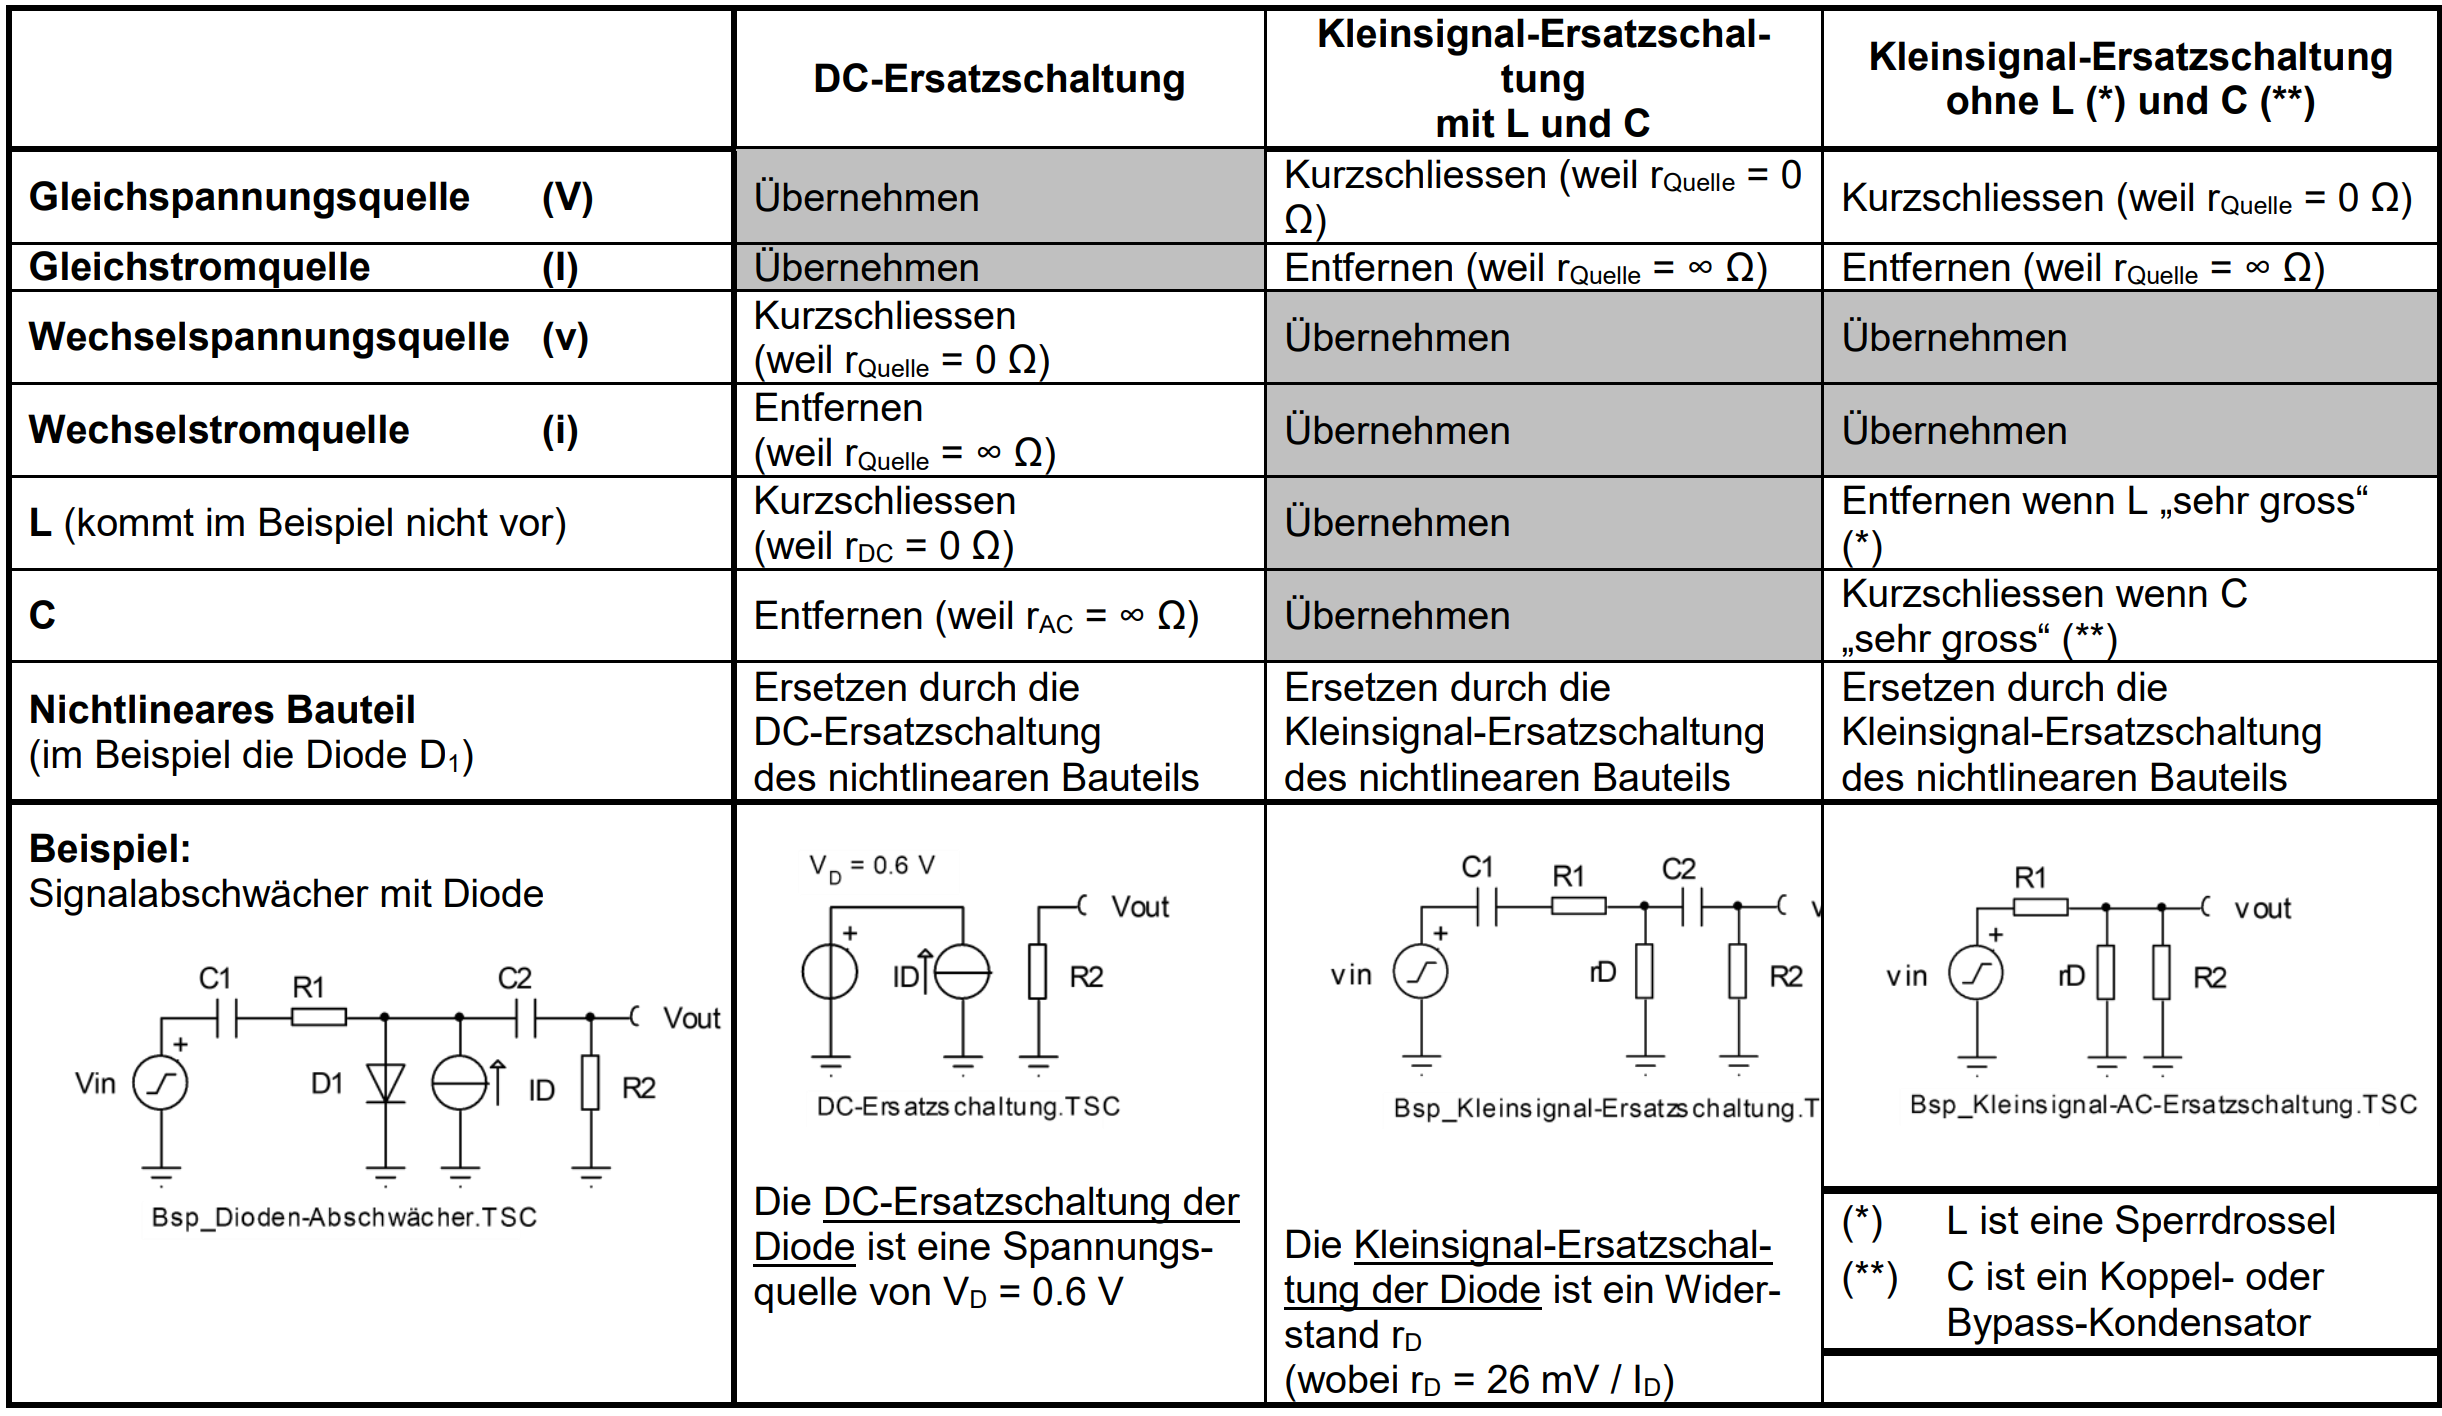
\includegraphics[width = 15cm]{img/Tabelle Kleinsignal Ersatzschaltung.png}
\newpage
\section{OpAmp}
\subsection{Schaltungen mit negativer Rückkopplung}
\begingroup
\small
\begin{tabularx}{0.8\textwidth}{p{155pt}p{155pt}p{155pt}}
  \textbf{Nicht Invertierender Verstärker}                                                          &
  \textbf{Invertierender Verstärker}                                                                &
  \textbf{Summierender Verstärker}                                                                    \\
  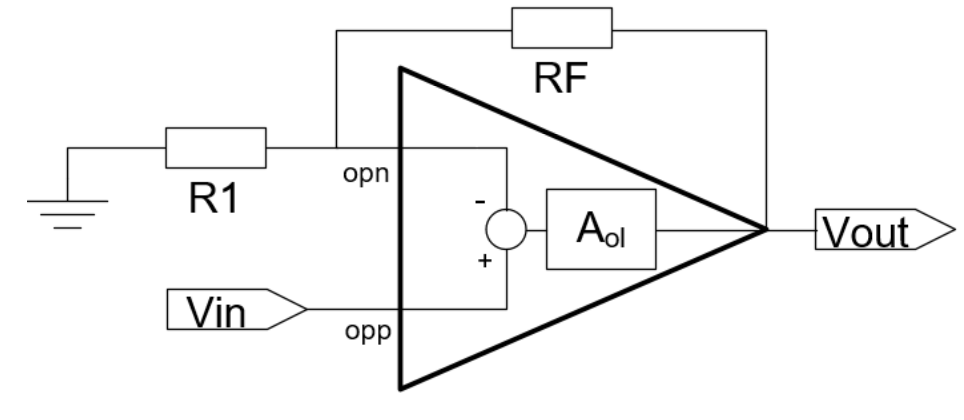
\includegraphics[width = 3.5cm]{img/OpAmp/Verstaerker_nicht_invertierend.png}                     &
  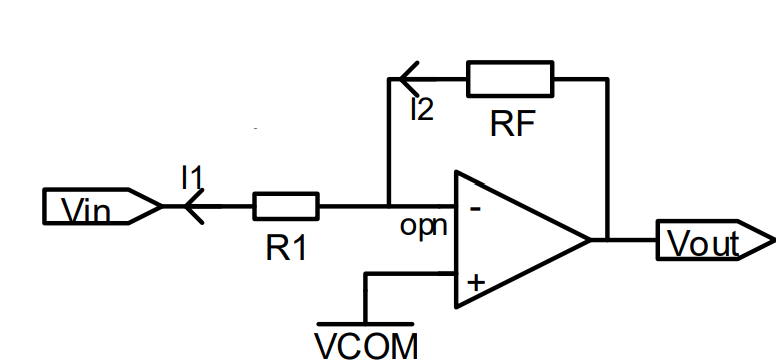
\includegraphics[width = 3.5cm]{img/OpAmp/Verstaerker_invertierend.png}                           &
  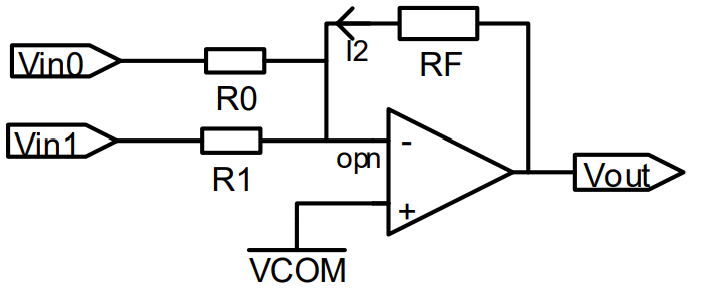
\includegraphics[width = 3.5cm]{img/OpAmp/Verstaerker_summierend.png}                               \\
  $ V_{out} = V_{in} \cdot (1 + \frac{R_F}{R_1})$                                                   &
  $ V_{out} = V_{RF} = -\frac{RF}{R_1}\cdot V_{in}$                                                 &
  $ V_{out} = RF \cdot I_2 = -RF \cdot (\frac{V_{in1}}{R_1} + \frac{V_{in0}}{R_0}) $                  \\
  \\
  \textbf{Buffer}                                                                                   &
  \textbf{Invertierender Addierer}                                                                  &
  \textbf{Gewichteter Subtrahierer}                                                                   \\
  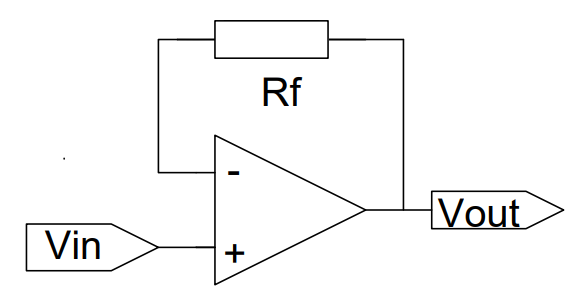
\includegraphics[width = 3.5cm]{img/OpAmp/Buffer.png}                                             &
  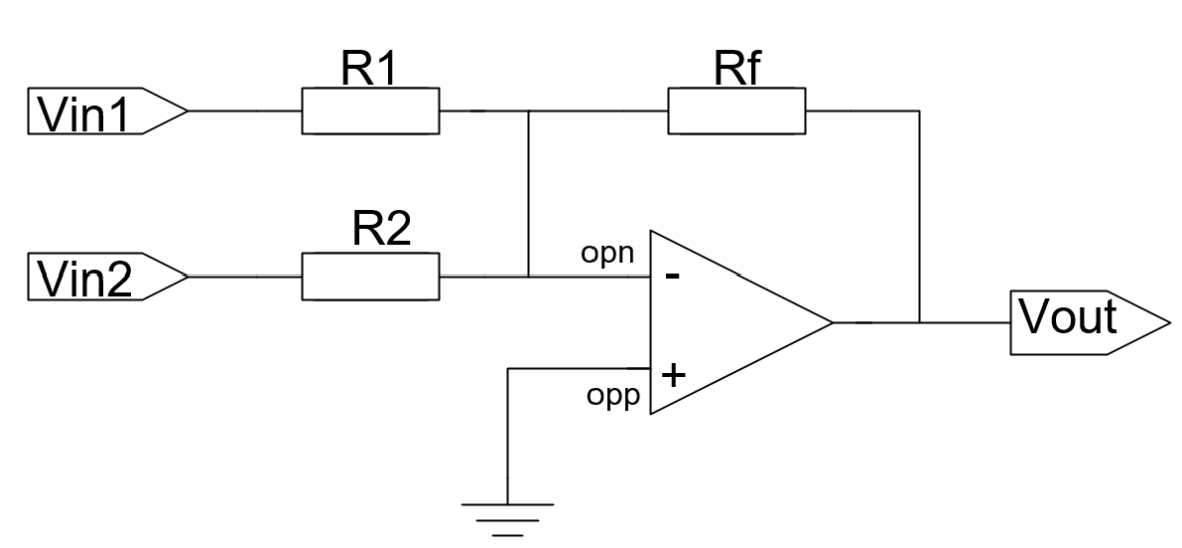
\includegraphics[width = 3.5cm]{img/OpAmp/Invertierender_Addierer.png}                            &
  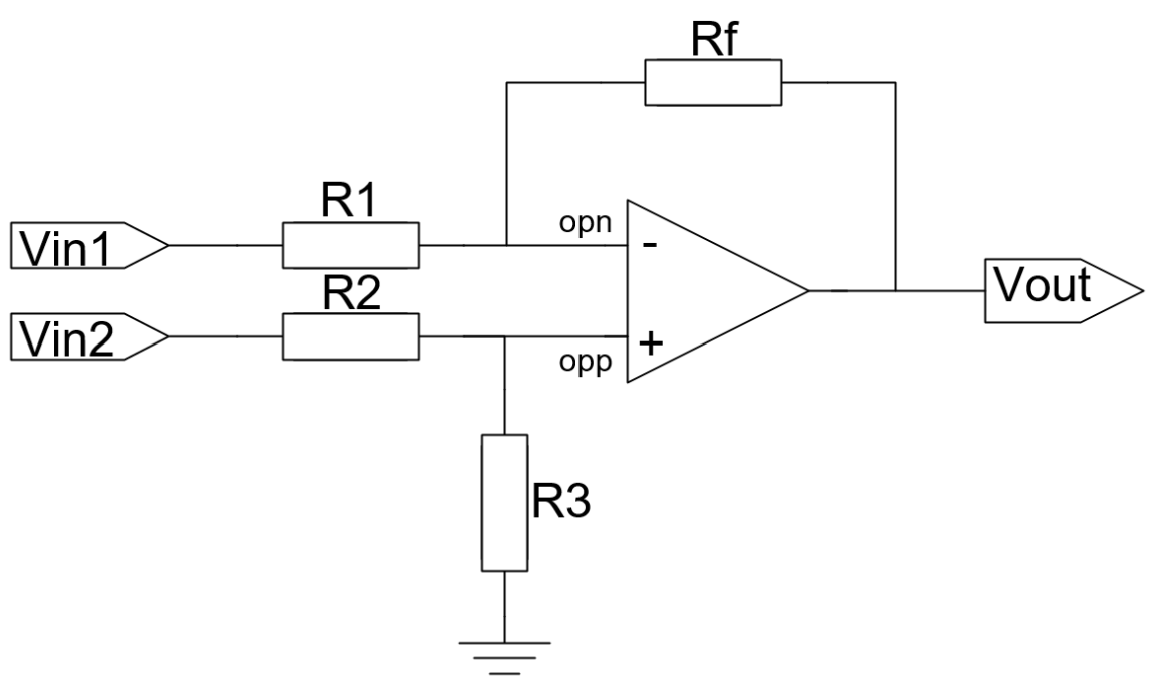
\includegraphics[width = 3.5cm]{img/OpAmp/Gewichteter_Subtrahierer.png}                             \\
  $ V_{out} = V_{in}$                                                                               &
  $ V_{out} = - RF \cdot (\frac{V_{in1}}{R_1} + \frac{V_{in2}}{R_2}) $                              &
  $ V_{out} =-\frac{RF}{R_1} \cdot V_{in1} $                                                          \\
  \\
  \textbf{Differenzverstärker}                                                                      &
  \textbf{Instrumentenverstärker}                                                                   &
  \textbf{Mehrstufige Verstärker}                                                                     \\
  \includegraphics[width = 3.5cm]{img/OpAmp/Differenzverstärker.png}                                &
  \includegraphics[width = 3.5cm]{img/OpAmp/Instrumentenverstärker.png}                             &
  \includegraphics[width = 3.5cm]{img/OpAmp/Mehrstufige_Verstärker.png}                               \\
  $ V_{out} = V_{AGND} + \frac{R_4}{R_3} \cdot(V_{in1} - V_{in2}) $                                 &
  $ V_{out} = V_{ref} + \frac{R_4}{R_3} \cdot (1 + \frac{Rf1 + Rf2}{RG}) \cdot (V_{in1} - V_{in2})$ &
  Verstärkung total $ A_{tot} = A_1 \cdot A_2 \cdot A_3\cdot\dots$                                    \\
  \\
  \textbf{Invertierender Verstärker \newline
  mit T-Glied in Rückkopplung}                                                                      &
  \textbf{Negativer Impedanz Konverter NIC}                                                           \\
  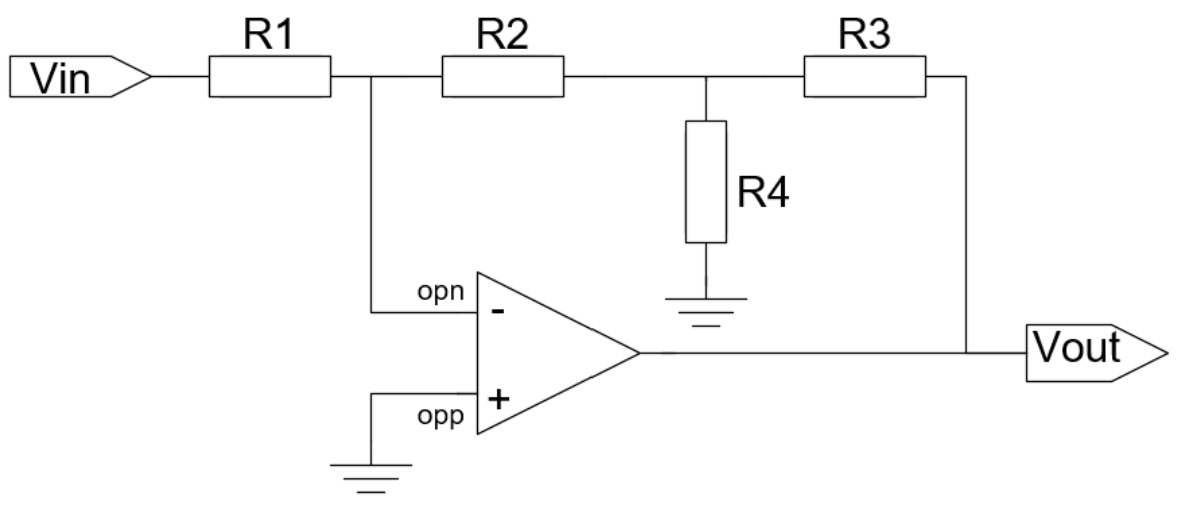
\includegraphics[width = 3.5cm]{img/OpAmp/Invertierender_Verstärker_mit_T-Glied_Rückkopplung.png} &
  \includegraphics[width = 3.5cm]{img/OpAmp/Negativer_Impedanz_Verstärker.png}                        \\
  $ V_{out} = - V_{in} \cdot \frac{R_2 + R_3 + \frac{R_2R_3}{R4}}{R_1} $
  \newline
  $ V_{out} = V_{in} \cdot (1+ \frac{R_2}{R_1})$                                                    &
  \\
\end{tabularx}
\endgroup

\subsubsection{Gesteuerte Quellen}
\begingroup
\small
\begin{tabularx}{0.8\textwidth}{p{100pt}p{100pt}p{100pt}p{120pt}}
  \textbf{Spannungsgesteuerte \newline Stromquelle V1}                                         &
  \textbf{Spannungsgesteuerte \newline  Stromquelle V2}                                        &
  \textbf{Spannungsgesteuerte \newline Stromquelle \newline
  für geerdete Last RL}                                                                        &
  \textbf{Stromgesteuerte \newline Stromquelle}                                                  \\
  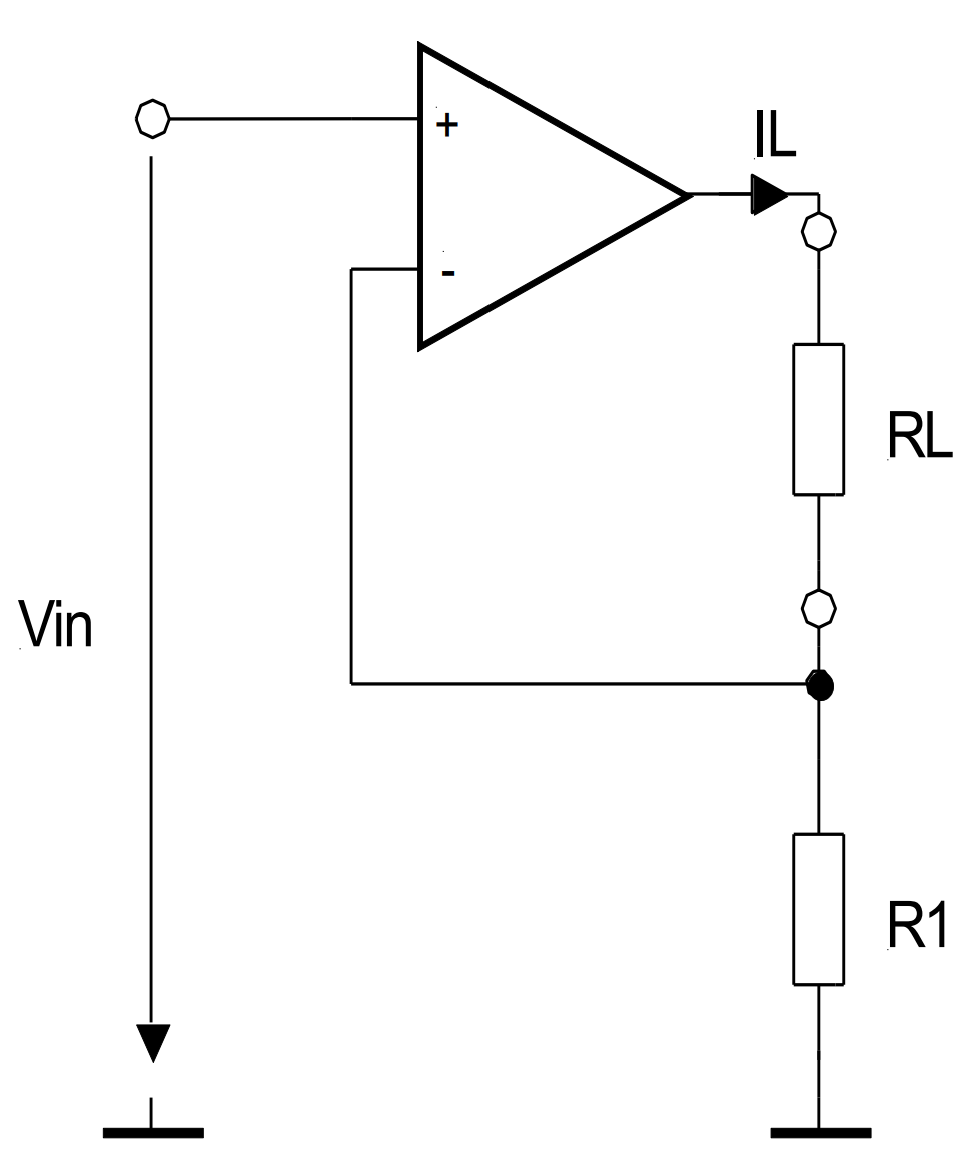
\includegraphics[width = 3.5cm]{img/OpAmp/Spannungsgesteuerte_Stromquelle_V1.png}            &
  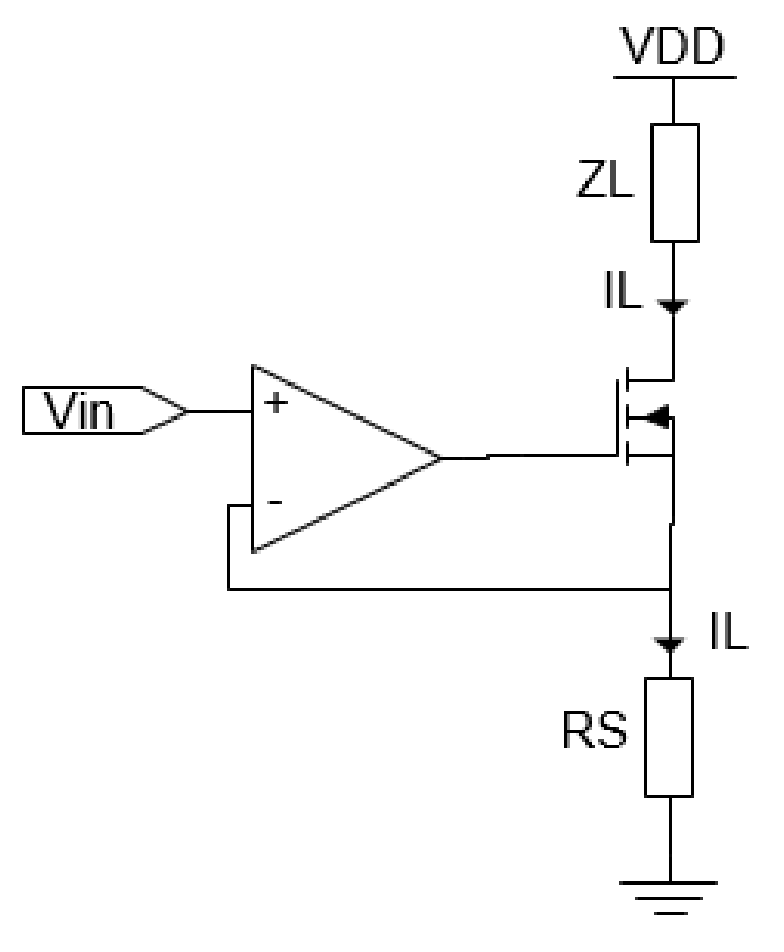
\includegraphics[width = 3.5cm]{img/OpAmp/Spannungsgesteuerte_Stromquelle_V2.png}            &
  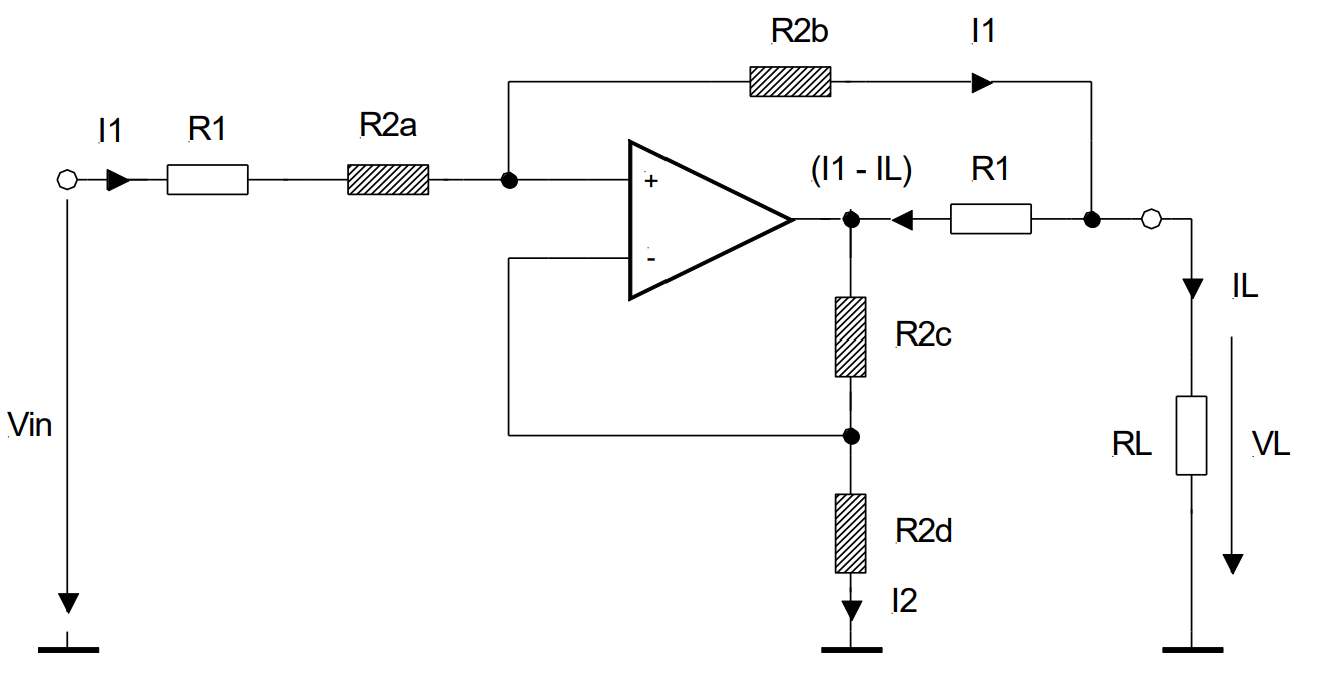
\includegraphics[width = 3.5cm]{img/OpAmp/Spannungsgesteuerte_Stromquelle_geerdete_Last.png} &
  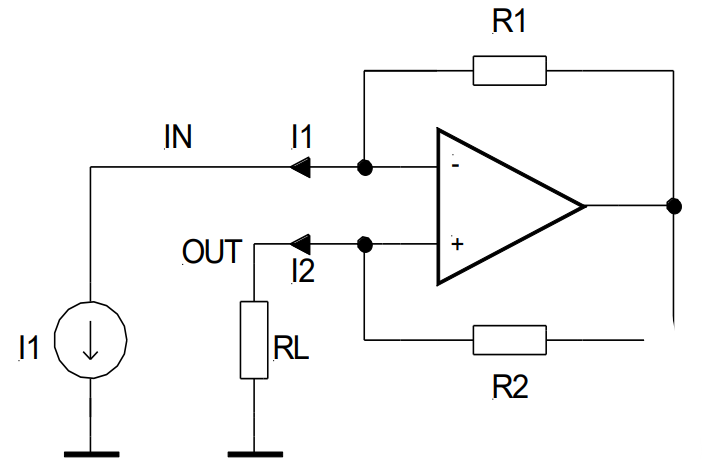
\includegraphics[width = 3.5cm]{img/OpAmp/Stromgesteuerte_Stromquelle.png}                     \\
  $ I_L = \frac{V_{in}}{R_1} $                                                                 &
  $ I_L = \frac{V_{in}}{R_S} $                                                                 &
  $ I_L = \frac{V_{in}}{R_1} $                                                                 &
  $ R_1I_1=R_2I_2; \; A_i = \frac{I_2}{I_1} = \frac{R_1}{R_2}  $
\end{tabularx}
\endgroup

\subsubsection{Filterschaltungen}
\begingroup
\small
\begin{tabularx}{\textwidth}{p{155pt}p{155pt}p{155pt}}
  \textbf{RC-Integrator}                                                                        &
  \textbf{Differenzierer}                                                                       &
  \textbf{Tiefpass-Filter}                                                                        \\
  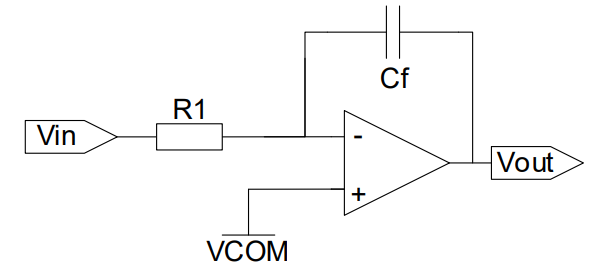
\includegraphics[width=3.5cm]{img/OpAmp/RC-Integrator.png}                                    &
  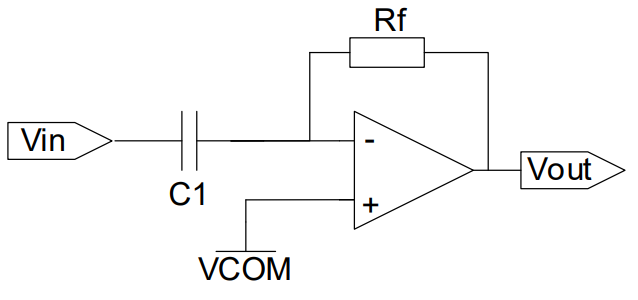
\includegraphics[width=3.5cm]{img/OpAmp/Differenzierer.png}                                   &
  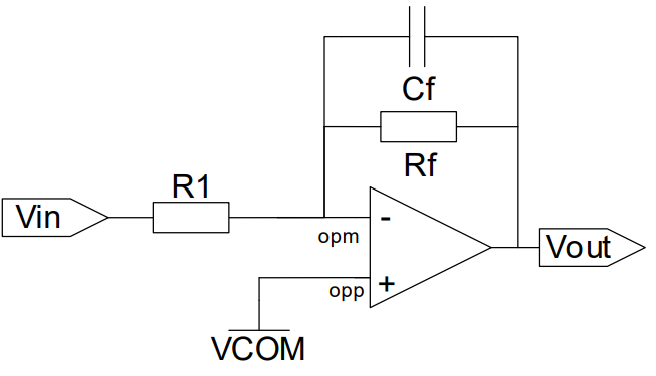
\includegraphics[width=3.5cm]{img/OpAmp/TiefpassFilter.png}                                     \\
  $V_{out}(t) = -\frac{1}{C} \int \limits _0 ^t i_c(\tau) d\tau + V_c(t=0)$
  \newline $V_{out}(t) = -\frac{1}{R \cdot C} \int \limits _0 ^t V_{in}(\tau) d\tau + V_c(t=0)$ &
  $V_{out} = -R_FC_1\frac{dv_{in}}{dt}$
  \newline  $i_c = C_1\frac{dv_c}{dt} = C_1\frac{dv_{in}}{dt} $                                 &
  Grenzfrequenz: $\frac{1}{2\pi R C} $
  \newline DC: $I_C = 0; \; V_{out} = -\frac{Rf}{R1}\cdot V_{in}$                                 \\
  \textbf{Bandpass-Filter}                                                                      &
  \textbf{Allpass-Filter}                                                                       &
  \\
  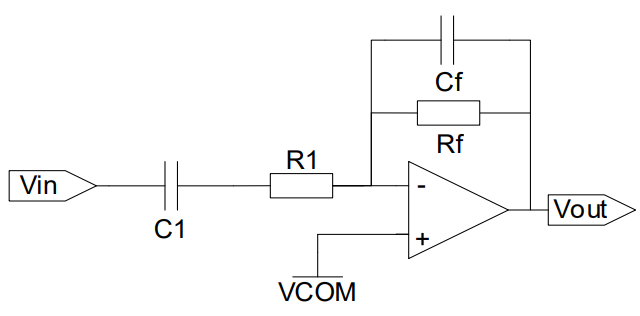
\includegraphics[width=3.5cm]{img/OpAmp/BandPass.png}                                         &
  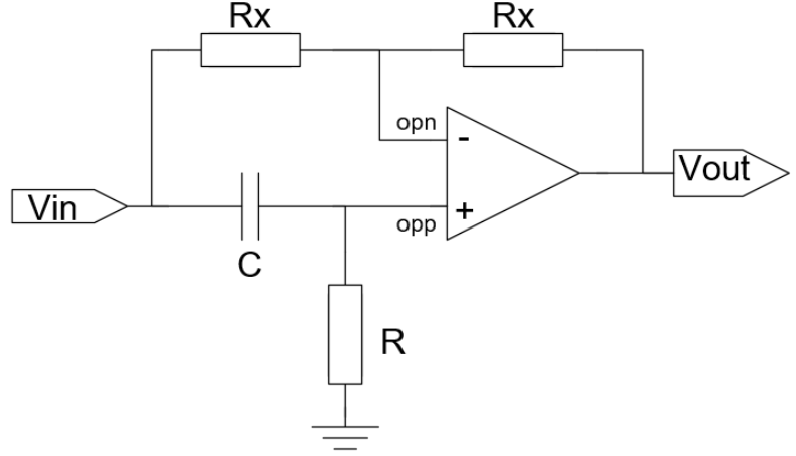
\includegraphics[width=3.5cm]{img/OpAmp/AllPass.png}                                          &
  \\
\end{tabularx}
\endgroup
\subsection{Nicht ideale OpAmps}
\begin{multicols}{2}
  \small
  \subsubsection*{Offset-Spannung \& Begrenzte Verstärkung}
  \begin{itemize}
    \item \textbf{Buffer}: \\
          $V_{out} = A_{ol} \cdot [(V_{in}+V_{os}) - V_{out}]$
          \\$[A_{ol}\gg 1$ : $V_{out} = V_{in} + V_{os}]$

    \item \textbf{Verstärker}: \\
          $V_{out} = \frac{A_{ol}}{1+A_{ol}\cdot\frac{R_1}{R_1+R_2}}\cdot(V_{in}+V_{os}) $
          \\$[A_{ol}\gg 1$: $V_{out} = \frac{R_1+R_2}{R_1}\cdot(V_{in}+V_{os})]$

    \item \textbf{Invertierender Verstärker}: \\
          $V_{out} = \frac{A_{ol}}{1+A_{ol}\cdot\frac{R_1}{R_1+R_2}}\cdot[(V_{AGND} + V_{os})-V_{in}\cdot\frac{R_2}{R_1+R_2}]$
          \\ $[A_{ol}\gg 1$: $V_{out} = \frac{R_1 + R_2}{R_1}\cdot(V_{AGND}+V_{os})-\frac{R_2}{R_1}\cdot V_{in}]$

    \item \textbf{Allgemein}: \\
          $V_{out} = \frac{R1 + R2}{R1}\cdot(V_{agnd}+R_{os})-\frac{R2}{R1}\cdot V_{in}$

  \end{itemize}
  \subsubsection*{Bias-Strom}
  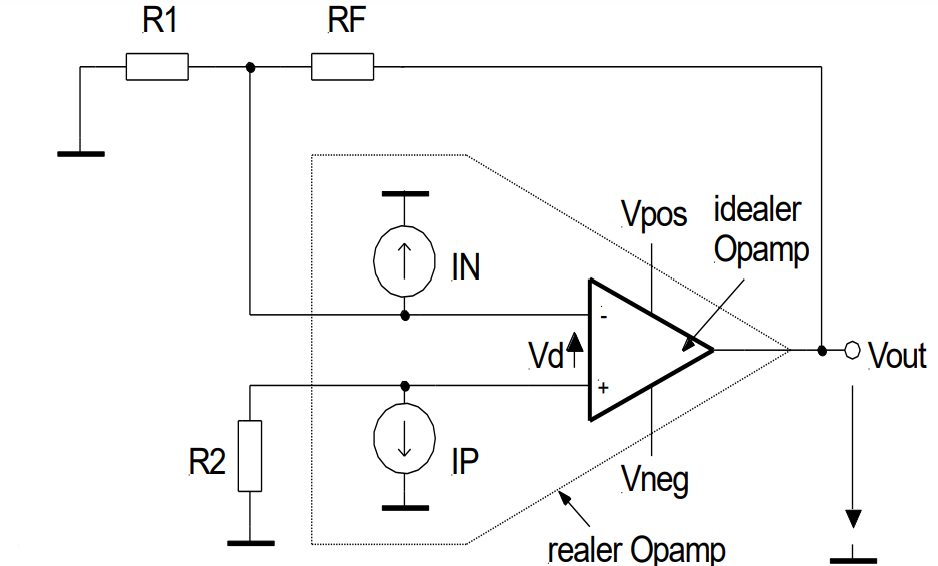
\includegraphics[height=3cm]{img/OpAmp/Fehler_Eingangsstrom.png}
  \tiny{Rechnung mit Superposition:}\\
  $V_{out E} = I_NR_F-R_2I_P(\frac{R_F+R_1}{R_1}) $\\
  \textbf{Offset-Strom}
  $V_{out E} = R_F\cdot(I_N-I_P) = R_F\cdot I_{OS}$
  \subsubsection*{Einganswiderstände}
  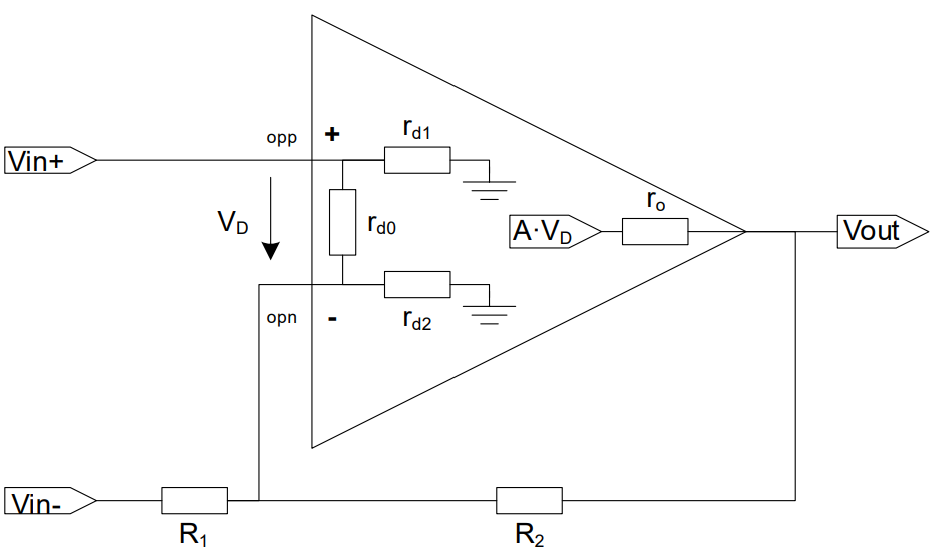
\includegraphics[height=3cm]{img/OpAmp/Fehler_Eingangswiderstand.png}\\
\end{multicols}

\begin{multicols}{2}
  \subsection{OpAmp als Komparator}
  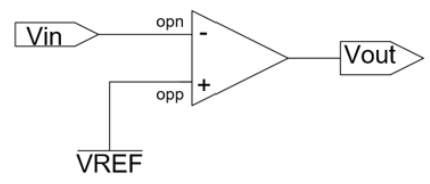
\includegraphics[width=3cm]{img/OpAmp/Komparator.png}\\
  $V_{out} = V_{mitte} = \frac{V_{pos} + V_{neg}}{2}$
  \subsubsection*{Schmitt-Trigger (nicht invertierend)}

  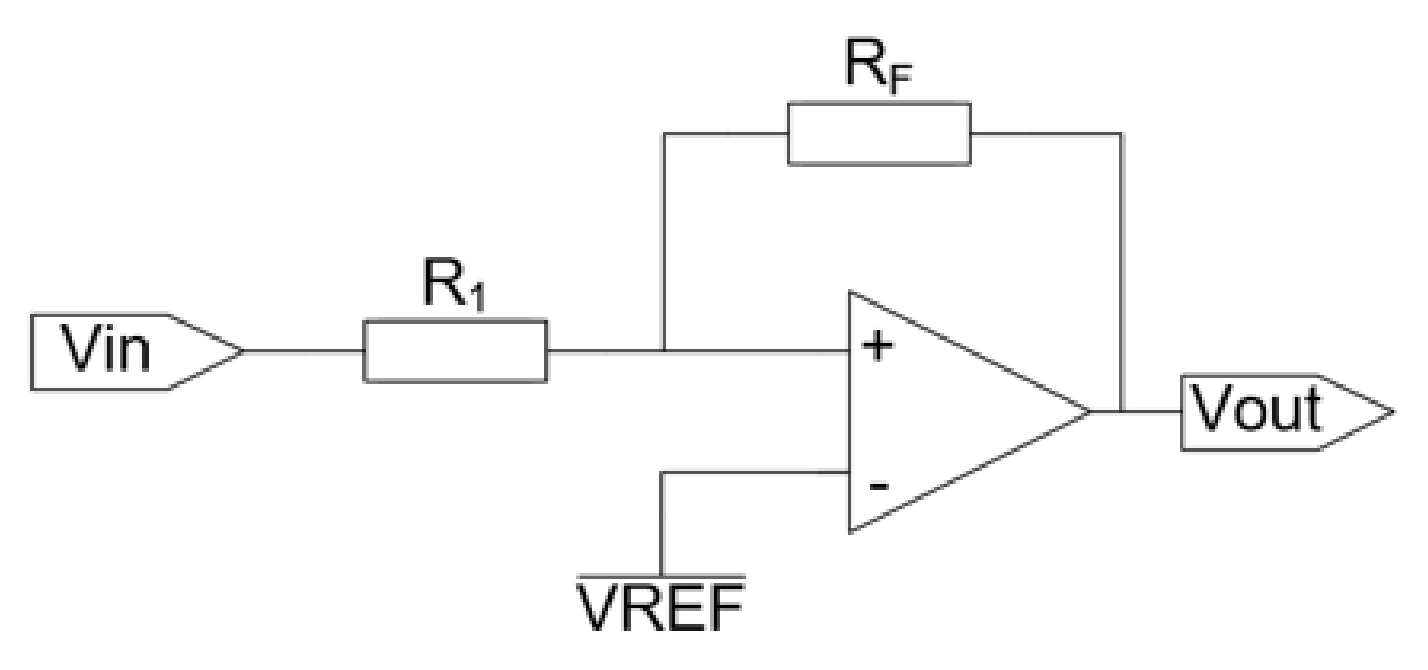
\includegraphics[width=3cm]{img/OpAmp/Schmitt-Trigger_nicht_invertierend.png}


  $V_{T_+} = V_{ref} + (V_{ref} - V_{out min})\frac{R_1}{R_F} $ \\
  $V_{T_-} = V_{ref} + (V_{out max} - V_{ref})\frac{R_1}{R_F} $\\
  $V_H = V_{T_+} - V_{T_-} = (V_{outmax} - V_{outmin})\frac{R_1}{R_F}$

  \subsubsection*{Schmitt Trigger (invertierend)}
  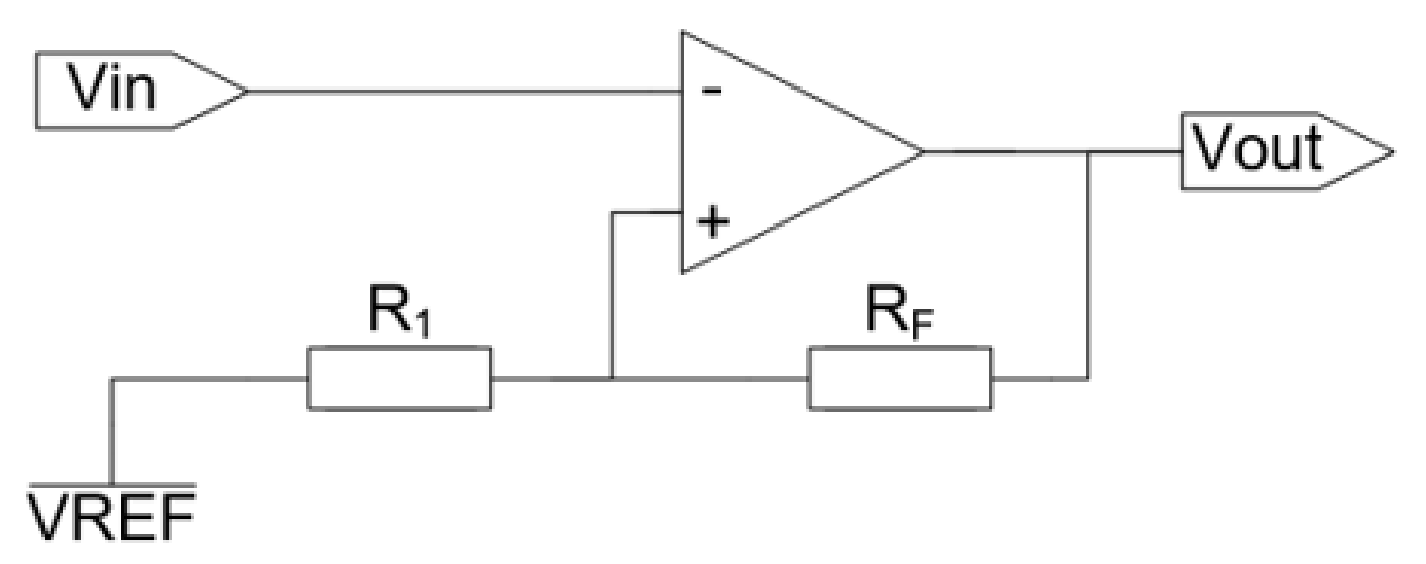
\includegraphics[width=4cm]{img/OpAmp/Schmitt-Trigger_invertierend.png}\\
  $V_{T_+} = V_{ref} + (V_{out max} - V_{ref})\frac{R_1}{R_1 + R_F} $ \\
  $V_{T_-} = V_{ref} + (V_{ref} - V_{out min})\frac{R_1}{R_1 + R_F} $\\
  $V_H = V_{T_+} - V_{T_-} = (V_{outmax} - V_{outmin})\frac{R_1}{R_1+R_F}$
\end{multicols}
\newpage
\section{Digital-/Analogwandler}

\begin{multicols}{5}


  \subsubsection*{Parallelverfahren}
  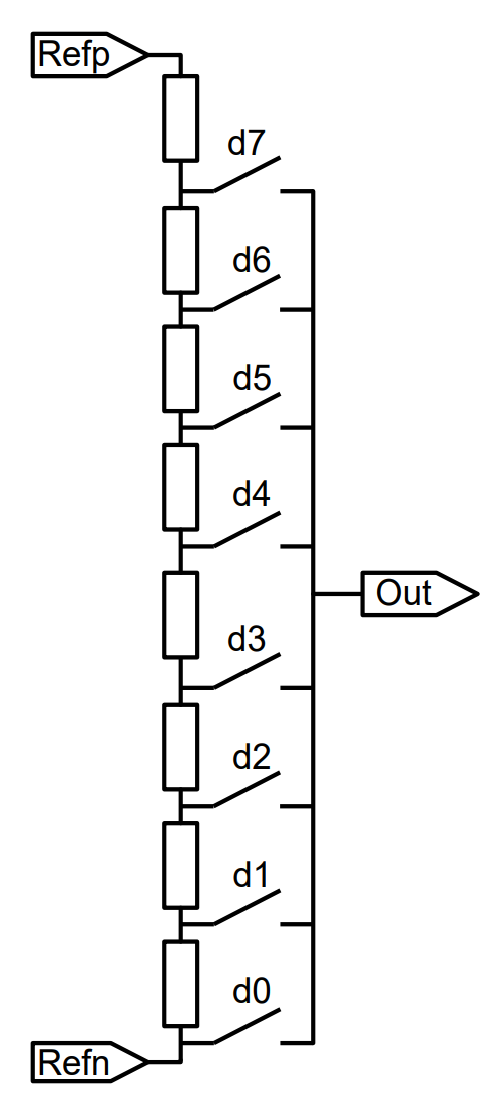
\includegraphics[height = 3cm]{img/DAC/Parallelverfahren.png}

  \subsubsection*{Wägeverfahren}
  \scriptsize
  \textbf{Spannung}
  \includegraphics[width = 3cm]{img/DAC/Wägeverfahren.png}
  \\\textbf{Strom}
  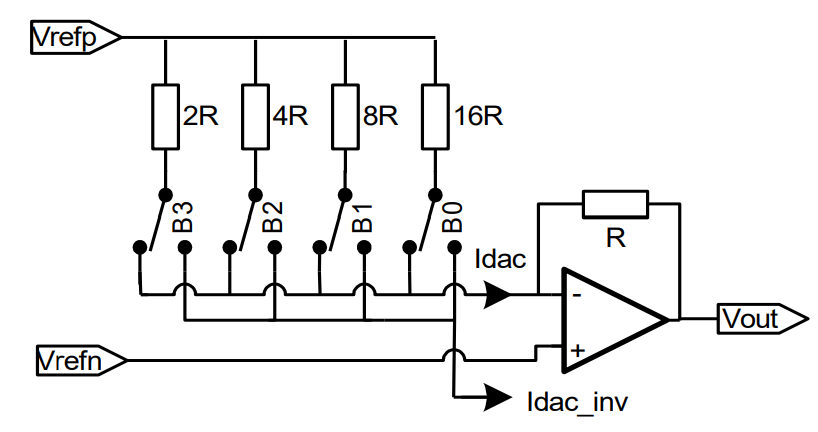
\includegraphics[width = 3cm]{img/DAC/Wägeverfahren_Ströme.png}
  \\\textbf{Kapazität}
  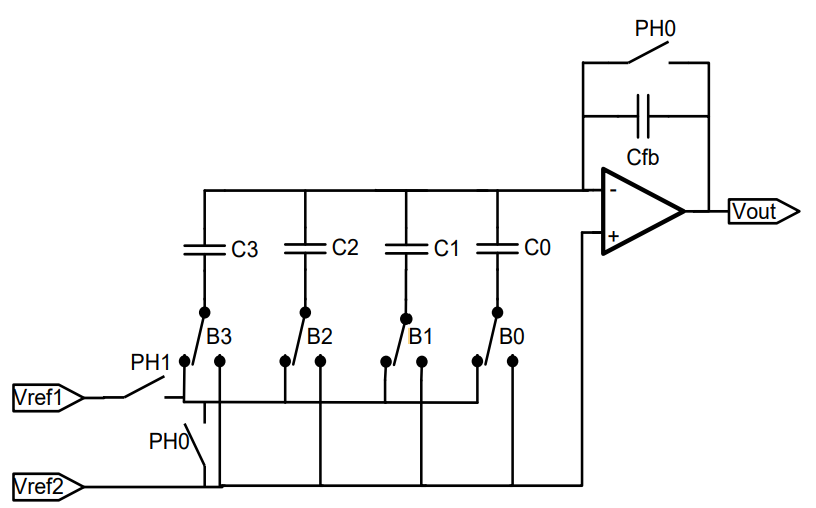
\includegraphics[width = 3cm]{img/DAC/C-DAC.png}
  \\\textbf{R-2R}
  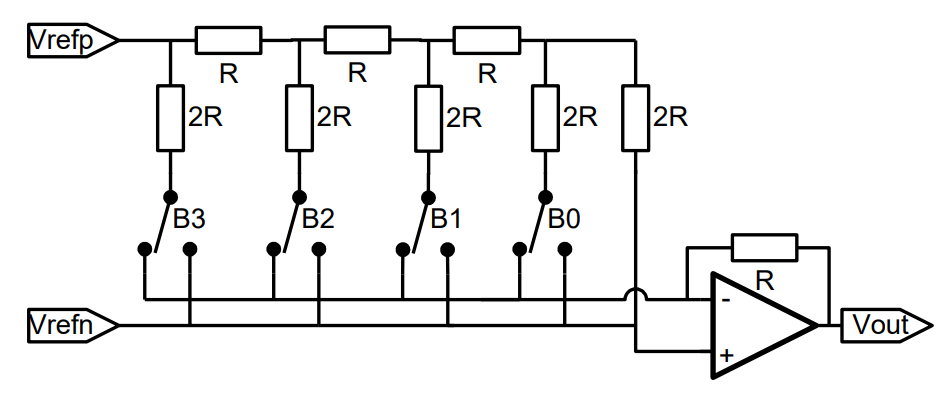
\includegraphics[width = 3cm]{img/DAC/R-2R-DAC.png}

  \subsubsection*{Zählverfahren}
  \scriptsize
  \textbf{PWM} \\
  \tiny{
    $\bar{V_{out} = V_{ref} \cdot \frac{n}{N}}$
    \\ Geglättete Ausgangsspannung ergibt DC}
  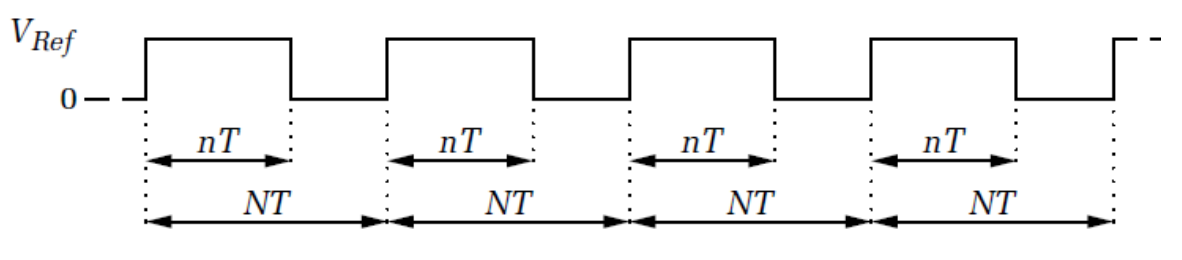
\includegraphics[width = 3cm]{img/DAC/PWM.png}
  \subsubsection*{Weitere Formen}
  \scriptsize
  \textbf{Kaskadiert}
  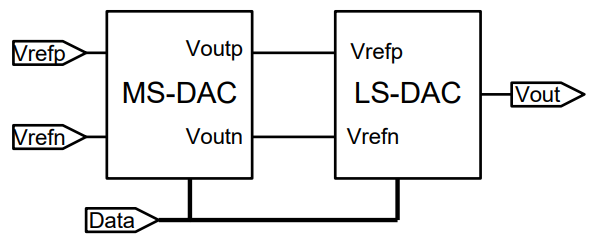
\includegraphics[width = 3cm]{img/DAC/Kaskadierte_Wandler.png}
  \\\textbf{Zyklisch}
  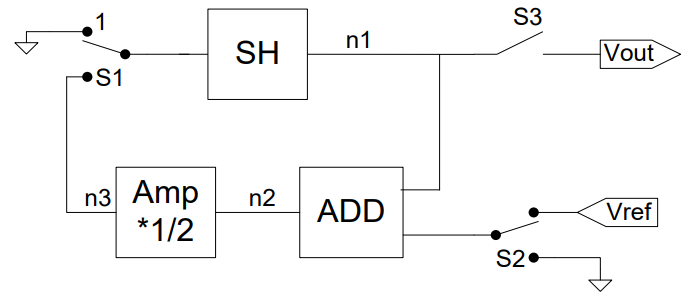
\includegraphics[width = 3cm]{img/DAC/Zyklischer_DAC.png}
  \\\textbf{Pipelined}
  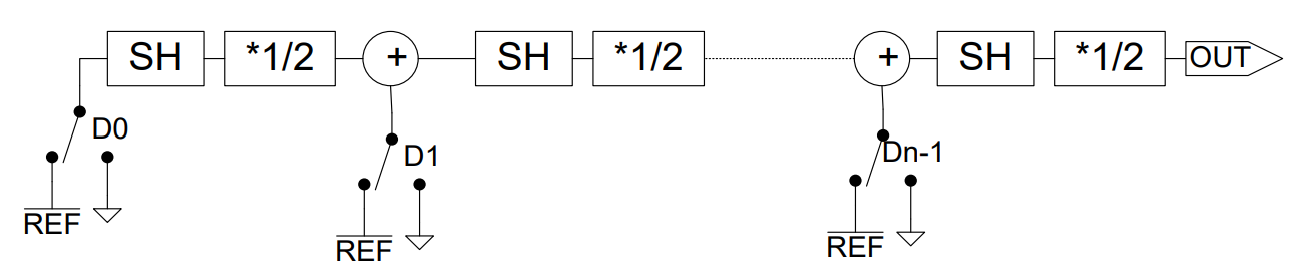
\includegraphics[width = 3cm]{img/DAC/Pipelined_DAC.png}
  \\\textbf{Mutliplizierend}
  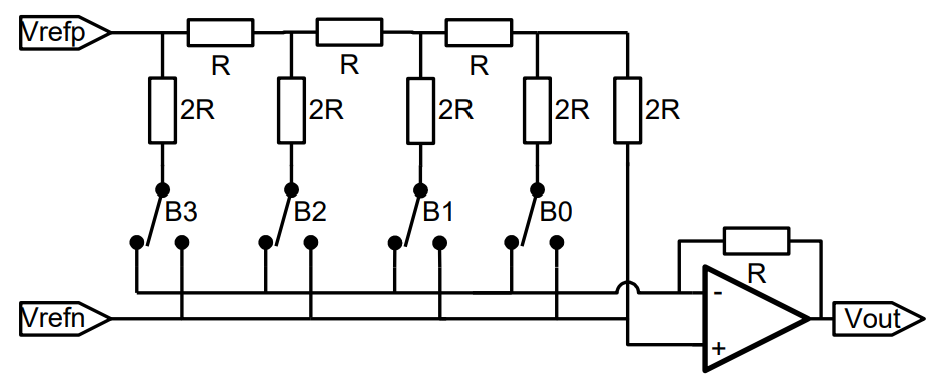
\includegraphics[width = 3cm]{img/DAC/Multiplizierender_Wanlder.png}
  \\\textbf{Exponentiell}
  \\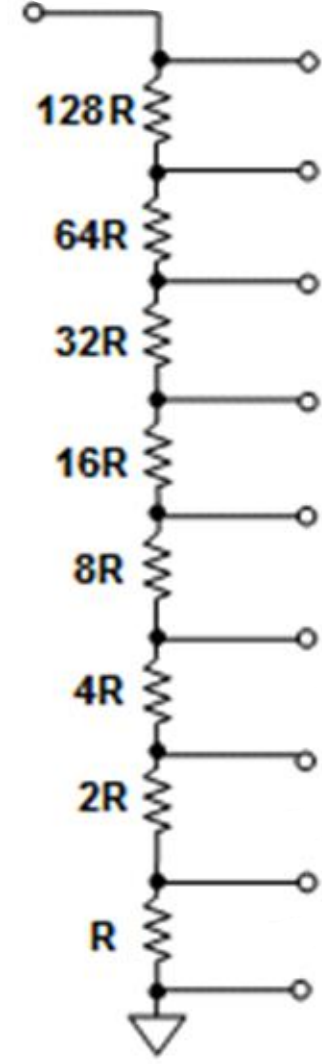
\includegraphics[height = 2cm]{img/DAC/Exponentieller_DAC.png}

  \normalsize
\end{multicols}
\subsubsection*{Fehler}
\begingroup
\small
\begin{tabularx}{\textwidth}{p{0.2\textwidth}p{0.2\textwidth}p{0.2\textwidth}p{0.2\textwidth}p{0.2\textwidth}}
  \textbf{Offset}
   &
  \textbf{Verstärkungsfehler}
   &
  \textbf{Integrale \newline Nichtlinearität}
   &
  \textbf{Differentielle Nichtlinearität}
   &
  \textbf{Verzögerungszeit}
  \\
  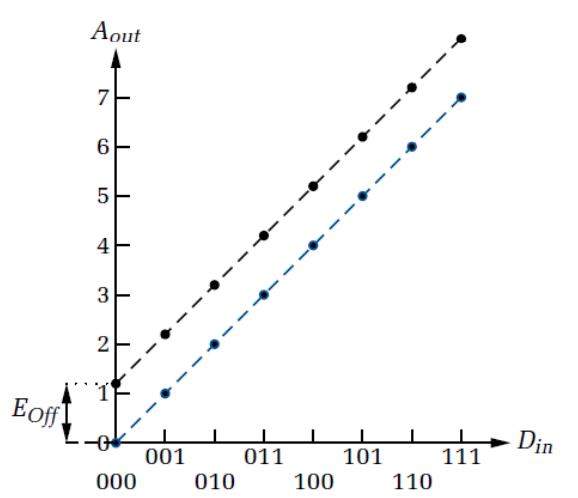
\includegraphics[width = 2cm]{img/DAC/Fehler/Offset.png}
   &
  \includegraphics[width = 2cm]{img/DAC/Fehler/Verstärkung.png}
   &
  \includegraphics[width = 2cm]{img/DAC/Fehler/IntegraleNichtlinearität.png}
   &
  \includegraphics[width = 2cm]{img/DAC/Fehler/DifferentielleNichtlinearität.png}
   &
  \includegraphics[width = 2cm]{img/DAC/Fehler/Verzögerungszeit.png}
\end{tabularx}
\endgroup





\end{document}
